\chapter{Literature Review}\label{chap:review}

\section{Citations and Bibliography}
This is supposed to be your literature review chapter. Instead, we look at ways to prepare the bibliography and citations instead. 

\section{The \texttt{*.bib} File}
First of all, bear in mind that your bibliography file (\verb|*.bib| files) is like a database like Mendeley.  That means you can maintain a centralised list, and reuse it for all your publications.  \LaTeX{} will only list sources that you actually cite in the text for each document, according to the bibliography and citation style you select in each document.  But you can still hack it so that your own publications are listed, even if you did not cite it. The order of the entry is not important. 
 

\begin{figure}[htb!]
\begin{lstlisting}[language={}]
@BOOK{latex:companion,
  title = {The {\LaTeX} Companion},
  publisher = {Addison-Wesley},
  year = {2004},
  author = {Frank Mittelbach and Michel Goosens and Johannes Braams and David Carlisle and Chris Rowley},
  series = {Addison-Wesley Series on Tools and Techniques for Computer Typesetting},
  address = {Boston, MA, USA},
  edition = {2nd}
}
\end{lstlisting}
\caption{A BibTeX Entry}\label{fig:bibtex}
\end{figure}

\clearpage	% I forced the next paragraph into new page
As an example, in \verb|mybib.bib| I created a Bib\TeX{} entry with JabRef and google scholar, the source text of which is shown in Figure~\ref{fig:bibtex}. Go to \url{https://scholar.google.com/}, click setting (on the left side of the page with three lines), click \verb|Show links to import citations into BibTeX| under the \verb|Bibliography manager| menu, and click \verb|Save|. 

\begin{figure}[htb!]\centering
	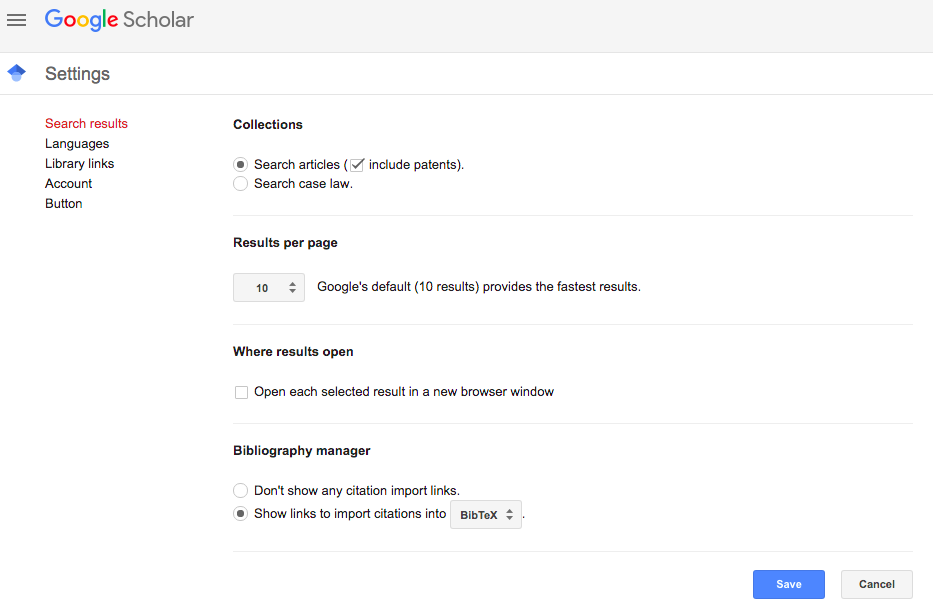
\includegraphics[scale=0.3]{googlescholar}
	\caption{Setting Google Scholar to show Import to BibTeX menu}\label{fig:googlescholar}
\end{figure}

One thing to note about authors' names: Bib\TeX{} recognises ``Mittelbach'' as the last name for both \texttt{Frank Mittelbach} and \texttt{Mittelbach, Frank}.  So for a name like ``Mohd Hanafi Mat Som'' and ``Lim Lian Tze'', you would have to specify it as \texttt{Mat Som, Mohd Hanafi} and either \texttt{Lian Tze Lim} or \texttt{Lim, Lian Tze} for Bib\TeX{} to recognise ``Mat Som'' and ``Lim'' as the last name correctly.  In addition, note that my surname (or family name) consists of multiple words, thus enclose it with braces to avoid surprises, like so: \texttt{Mohd Hanafi \{Mat Som\}}.

\section{Citations using the \texttt{natbib} package}
The \verb|unimapcgsfyp| class imports the \verb|natbib| package which provides citation mechanism as per required by the CGS (and School), so see its documentation for more details.  On a MiK\TeX{} installation,
% it should be in \url{texmf/doc/latex/natbib/natbib.dvi} or \url{natbib.pdf}, in the path where you installed MiKTeX. 
use the command prompt to issue \lstinline|mthelp --view natbib| to access the documentation.
On TeXLive, simply type \verb|texdoc natbib| and the documentation will be displayed automatically, if it's found on your machine.

The basic citation commands are \verb|\citet| and \verb|\citep|, which stands for \emph{textual} and \emph{parenthetical} citation respectively.  They take extra arguments, too, for adding notes in the citations.  Please refer to the \verb|natbib| manual \url{http://texdoc.net/texmf-dist/doc/latex/natbib/natbib.pdf} \cite{cgs:thesis:guideline:2017,latex:companion,lim:2007,lim:latextypesetting}. 

\subsection{IEEE Citation Style}
The default for FYP bibliography style is IEEE:

\begin{itemize}[nosep]\singlespacing
	\item \verb|\citet{latex:companion}| $\to$ \citet{latex:companion}
	\item \verb|\citep{latex:companion}| $\to$ \citep{latex:companion}
	\item \verb|\citet{latex:companion,roberts}| $\to$ \citet{latex:companion,roberts}
	\item \verb|\citep{latex:companion,roberts}| $\to$ \citep{latex:companion,roberts}
	\item \verb|\citet[chap.~2]{latex:companion}| $\to$ \citet[chap.~2]{latex:companion}
	\item \verb|\citep[chap.~2]{latex:companion}| $\to$ \citep[chap.~2]{latex:companion}
\end{itemize}

You may also want to write only the author's name or year occassionally:

\begin{itemize}[nosep]\singlespacing
	\item \verb|\citeauthor{latex:companion}| $\to$ \citeauthor{latex:companion}
	\item \verb|\citeyear{latex:companion}| $\to$ \citeyear{latex:companion}
\end{itemize} 

\subsubsection{Change citation format}

You may want to change the citation format for example in literature review table. See Table~\ref{tab:longtable} in Chapter~\ref{chap:methodology}. This can be achieved using \verb|\setcitestyle{authoryear,round}|. For more information please see the \verb|natbib| documentation. 

\begin{itemize}[nosep]\singlespacing
	\item \verb|\citet{latex:companion}| \\ $\to$ \citet{latex:companion}
	\item { \setcitestyle{authoryear,round} \verb|\citet{latex:companion} {\setcitestyle{authoryear,round} }| \\ $\to$ \citet{latex:companion} } 
	\item \verb|\citet{latex:companion}| \\ $\to$ \citet{latex:companion}
\end{itemize}

\subsection{Entry Types}

This section give some examples of entry of references. There references are formatted according to IEEE style \citep{ieee}. 

\begin{itemize}[nosep]\singlespacing
	\item Journal (\verb|@article|): \citet{othman2019effect} 
	\item Proceeding/Conference (\verb|@inproceedings|): \citet{wanna2018fracture} found that... 
	\item Book (\verb|@book|): As mentioned earlier \citep{latex:companion} 
	\item Internet Sources (\verb|@misc|): As mentioned earlier \citep{lim:latextypesetting} 
\end{itemize}